


\begin{abstract}[\hspace*{-10pt}]
    This chapter draws mainly on the published work: \fullcite{baillie_bayesian_2025}  % Ce chapitre reprend principalement les travaux publiés dans: 
\end{abstract}

\begin{abstract}
Estimating seismic fragility curves under conditions of limited data and binary structural responses remains a challenge that is commonly addressed using Bayesian inference to update a probit-lognormal modeling of fragility curves.
% Building on the reference prior theory to ensure 
Since the prior selection remains a critical step in such a context, we aim at constructing in this chapter a prior that (i) minimizes the subjectivity it embeds, and (ii) is robust in terms of generation of irregular estimates (such as unit-step functions).
To do so, we introduce 
a constrained reference prior that is designed to regularize the posterior distribution while conserving an objective characteristic.
Two implementation strategies are explored: a numerical approximation of the constrained prior density and a variational approximation using a neural network that implicitly parameterizes the prior. %trained to maximize mutual information. 
We compare both approaches through synthetic examples and a real case study.
Our results highlight the capacity of the constrained prior to provide accurate and efficient estimates.
% ur results show the usefulness of this approach in recovering the target distribution.
%, highlighting the trade-offs between computational cost and estimation quality. An appendix further examines the impact of neural network architecture on the variational method’s performance.
%
\end{abstract}

\minitoc


\section{Introduction}

% The estimation of seismic fragility curves 

In the seismic probabilistic risk assessment (SPRA) framework, the estimation of seismic fragility curves is a critical step. 
We recall that those curves are defined in   \cref{chap:frags-intro}, where we review the methods that are used in the literature to estimate them.
As a matter of fact, the information provided in the available databases to estimate the fragility curves is sometimes poor.
In our study, we are particularly interested in cases where
(i) the data are scarce, and (ii) the available knowledge about the mechanical system's response to the seismic excitation is limited to a binary outcome (i.e., failure or non-failure).
Under those settings, the parameterization of the fragility curve using the probit-lognormal model is a widely recognized approach in earthquake engineering.




% The information provided in the statistics 


The Bayesian framework has been widely implemented for estimating probit-lognormal seismic fragility curves of mechanical structures and components. %(see   \cref{chap:frags-intro} for a complete review of seismic fragility curve estimation techniques).
As a matter of fact, this framework has been proven efficient over classical frequentist methods in avoiding the generation of irregular estimates ---such as unit-step functions--- that may arise when limited numbers of data are available.

The common 
weaknesses of most of these approaches result from  %lies in 
their prior construction processes.  
Indeed, on the one hand, informative priors may be efficient but need to be 
avoided in reliability assessment studies because of the subjectivity they embed.
% in reliability studies since
On the other hand, the work conducted in   \cref{chap:prem} demonstrates that (i) insufficiently informative priors do not guarantee to produce proper posteriors given the likelihood decay rates of the probit-lognormal model, and that (ii)  
the reference prior is, most of the time, and in particular for the probit-lognormal model, defined by considering that the data are not what we call ``degenerate''. % (section 8.5).
%
%the reference prior for this model is limited to 
%case studies where the data are not what we call ``degenerate''. %The degeneracy is defined when, in the observed data, the failures and non-failures can be classified 
% namely which
% are partitioned into two disjoint subsets when classified according to IM values: the subset for
% which there is no failure and the other one for which there is failure, 
That degeneracy phenomenon represents a major curse when estimating seismic fragility curves, and the work done in   \cref{chap:prem} shows that is does not only affect the Bayesian estimates. Frequentist methods such as MLE when coupled with bootstrap techniques are also very affected.
Moreover, in   \cref{app:chap:uncecomp}, we illustrate on an example that this degeneracy is likely to occur (i) under small samples, and (ii) when the IM that is considered is more correlated with the structure's response.
The latter statement paradoxically jeopardizes the estimation of the fragility curve given an input that embeds more information on the output. % more correlated IM to the structure's response ---such as the PSA--- 









%Indeed, low informative prior are not guaranteed to issue proper posteriors given the weak decay rates of the likelihood of the probit-lognormal model (we refer to   \cref{chap:prem} where these decay rates are elucidated).
%On the other hand, informative priors are not affected by this issue, but need to be avoided in some reliability studies since the trustworthiness of their posterior estimate is jeopardized by the subjectivity they embed.
%Reference priors have been proven more robust than the latter two in   \cref{chap:prem}, yet their use remains limited to case study where the data is not ``degenerate''.
%That degeneracy was defined in \cref{chap:prem} 


%Additionally, the results in   \cref{app:chap:uncecomp} elucidate the paradoxical curse provided by the degeneracy. 
%It makes the estimation considering an IM more correlated with the structure's response less efficient.



%That praised capability to ``regularize'' the estimates is actually limited. Indeed, in   \cref{chap:prem}, we proved that the decay rates of the probit-lognormal likelihood sometimes does not shrink in some particular direction of the paramters' space under some  when the observed data are empirically 


In this chapter, we propose a truly regularizing objective prior based Bayesian methodology, in the sense that the prior we propose is sought to avoid the generation of unrealistic fragility curves ---even in degenerate scenarios--- while conserving an objective characteristic (as much as possible).
% being preserved from too much subjective thought introduction.
% For this s
When looking for objective priors, we recall that the reference prior theory is prominent, since it suggests constructing priors that maximize the mutual information,  which amounts maximizing the information brought by the data to the posterior (we refer to   \cref{chap:intro-ref} for a complete review of the reference prior theory).
In this study, we
mainly rely on the theoretical work developed in   \cref{chap:constrained-prior}, which suggests incorporating constraints to the reference prior. %(we recall that the reference prior theory was reviewed in   \cref{chap:intro-ref}).
The constraints %incorporation suggested
take the form of linear constraints that slightly regularize the reference prior's decay rate to ensure it yields proper posteriors.
%does not alter too much the prior.


%The objective of this work is 
To implement the constrained reference prior, we compare two methodologies.
The first one consists in approximating numerically the prior density by interpolating the integrals involved in its theoretical non-explicit formulation. %\emph{A posteriori} samples can be obtained 
This approach corresponds to the one conducted in   \cref{chap:prem} with the unconstrained reference prior. It has the disadvantage of being computationally expensive.
The second methodology consists in using a variational approximation of the reference prior (VA-RP).
This method consists in applying the algorithm constructed in   \cref{chap:varp}, which parameterizes the reference prior as the output of a neural network.
The weights of the neural networks are trained to maximize the mutual information, while ensuring the incorporated constraint on the prior is satisfied.
In this study, the neural network architecture is specifically tailored to the context of seismic fragility curves estimation.
In both methods, we assess the performance of the posterior distributions, which are estimated using Markov Chain Monte-Carlo (MCMC) techniques.


After this introduction, we briefly recall the probit-lognormal modeling of % of the probit-lognormal model of 
fragility curves. Then, we derive the theoretical expression of a constrained reference prior in \cref{sec:constr-frags:constrained}.
This expression is non-explicit, yet we explain how it can be used to numerically approximate the prior's density.
In \cref{sec:constr-frags:varp}, we propose a second approach that is based on variational inference to approximate the constrained reference prior.
The two approaches are then compared in \cref{sec:constr-frags:coparisonpriors}, before being applied on a real case study in \cref{sec:constr-frags:appasg}.
Before to conclude, we propose some results in an appendix (\cref{sec:constr-frags:app}) to provide more insight about the impact of the neural network's architecture on the variational approximation of the reference prior.



%We also explain how 
%This theoretical expression can be used 



%propose a linear constraint


\section{Reminder of the probit-lognormal model and of the Bayesian framework}\label{sec:constr-frags:model}


We remind that the probit-lognormal model was defined in   \cref{chap:frags-intro}. It consists in a statistical model where the data take the form of realizations of the random vector $Y=(Z,A)$, where $A\in\cA\subset(0,\infty)$ refers to the IM of the seismic signal, and $Z\in\{0,1\}$ refers to the outcome ($Z=1$ in case of a failure, $Z=0$ otherwise). The model consists in considering
the following parameterized distribution of $Y$ conditionally to $\theta=(\alpha,\beta)\in\Theta$:
    \begin{equation}
        A\sim A|\theta\sim H,\quad\text{and}\quad Z|A,\theta\sim\cB(P_f(A)),
    \end{equation}
where $H$ is the distribution of the IM, $\cB(p)$ denotes the Bernoulli distribution of parameter $p$, and $P_f$ refers to the probit-lognormal fragility curve:
\begin{equation}
    P_f(a) = \PP(Z=1|\text{IM}=a,\,\theta) = \Phi\left(\frac{\log a-\log\alpha}{\beta}\right),
\end{equation}
with $\Phi$ being the c.d.f. of a standard Gaussian distribution. This model is parameterized by the two parameters $\alpha\in(0,\infty)$ and $\beta\in(0,\infty)$, namely the median and the log standard deviation. 

%The model admits the following likelihood:
Given $k$ realizations $(\mbf z^k,\mbf a^k)$ of $Y$ ($\mbf z^k=(z_i)_{i=1}^k$ and $\mbf a^k=(a_i)_{i=1}^k$), the likelihood of this model is
\begin{equation}\label{eq:constr-frag:likelihood}
    \ell_k(\mbf z^k|\mbf a^k,\theta) = \prod_{i=1}^k\ell(z_i|a_i,\theta) = \prod_{i=1}^k\Phi\left(\frac{\log a_i-\log\alpha}{\beta}\right)^{z_i}\left(1-\Phi\left(\frac{\log a_i-\log\alpha}{\beta}\right)\right)^{1-z_i}.
\end{equation}





% The Bayesian framework 

We recall that incorporating the Bayesian framework in this model amounts to choose a prior on $\theta$ whose density is denoted by $\pi$.
% From a prior on $\theta$ whose density is $\pi$
% This way it is possible
It allows to define a posterior whose density $p(\cdot|\mbf z^k,\mbf a^k)$ is given by the Bayes' theorem:
\begin{equation}\label{eq:constr-frag:posterior}
    p(\theta|\mbf z^k,\mbf a^k) = \frac{\ell_k(\mbf z^k|\mbf a^k,\theta)\pi(\theta)}{\int_{\Theta}\ell_k(\mbf z^k|\mbf a^k,\theta')\pi(\theta')d\theta'}.
\end{equation}
Note that if the integral in the above equation is finite, then the posterior has to be proper. If it is not, it is still possible to define the posterior up to a multiplicative constant (see   \cref{chap:intro-ref}), but it does not permit to generate \emph{a posteriori} samples of $\theta$ for inference anymore.




\subsubsection{Degeneracy of the likelihood}

We recall below the asymptotic decay rates of the model's likelihood, that are derived in   \cref{chap:prem}:
\begin{align}
    \forall\alpha>0,\, \ell_k(\mbf z^k|\mbf a^k,\theta) &\conv{\beta\rightarrow\infty}2^{-k}\quad\text{and}\quad
    % \end{equation}
% and
    % \begin{equation}
        \ell_k(\mbf z^k|\mbf a^k,\theta) \aseq{\beta\rightarrow0}O\left(\beta^{|\mbf N|}e^{-\frac{\mbf N^T\log^2\frac{\mbf a^k}{\alpha}}{2\beta^2}}\right) ,\\
    \forall\beta>0,\, \ell_k(\mbf z^k|\mbf a^k,\theta)  &\aseq{\alpha\rightarrow0}  O\left(|\log\alpha|^{|\mbf z^k|-k} e^{-\frac{1}{2\beta^2}\sum_{i=1}^k (1-z_i)(\log a_i-\log\alpha)^2} \right),\\
    \ell_k(\mbf z^k|\mbf a^k,\theta) &\aseq{\alpha\rightarrow\infty}  O\left(\log(\alpha)^{-|\mbf z^k|} e^{-\frac{1}{2\beta^2}\sum_{i=1}^k z_i(\log a_i-\log\alpha)^2} \right) ,
\end{align}
where $\mbf N=(z_i\indic_{a_i<\alpha}+(1-z_i)\indic_{a_i>\alpha})_{i=1}^k$, $\log^2\frac{\mbf a^k}{\alpha}=(\log^2\frac{a_i}{\alpha})_{i=1}^k$, 
    $|\mbf N|=\sum_{i=1}^kN_i$ and
    $|\mbf z^k|=\sum_{i=1}^kz_i$. %is the number of failures in the observed sample.

% Several points must be considered 
%
These formulas indicate that the likelihood asymptotic behavior may drastically change given different data samples $(\mbf z^k,\mbf a^k)$.
This remark leads to the definition of degeneracy of the likelihood, expressed below.


\begin{defi}[Likelihood degeneracy]\label{def:constr-frag:degeneracy}
    %If the observed data $(\mbf z^k,\mbf a^k)$ are such that, either,
    If the observed samples $(\mbf z^k,\mbf a^k)$ belong to one of the following three types:
    \begin{itemize}
        \item
        type 1 : no failure is observed: $z_i=0$ for any $i$;
        \item type 2 : only failures are observed: $z_i=1$ for any $i$;
        \item type 3 : the failures and non-failures are partitioned into two disjoint subsets when classified according to their IM values:
        %the failures and successes are discriminated according to their IM: 
        there exists $a\in\cA$ such that for any $i,j$, $a_i<a<a_j\Longleftrightarrow z_i\ne z_j$ (see the illustration in \cref{fig:constr-frags:degenerate-frag});
    \end{itemize}
    then the likelihood is degenerate.
\end{defi}


\begin{figure}[h]
    \centering
    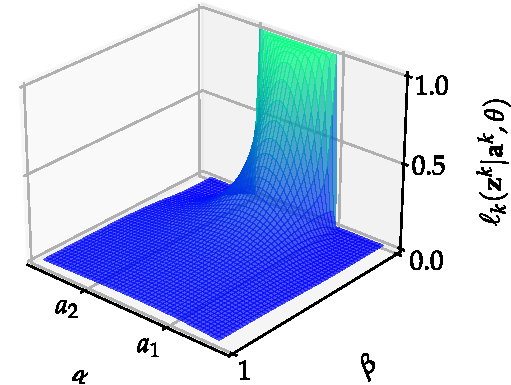
\includegraphics[width=4.6cm]{figures/PREM/likelihood_degen.pdf}\qquad
    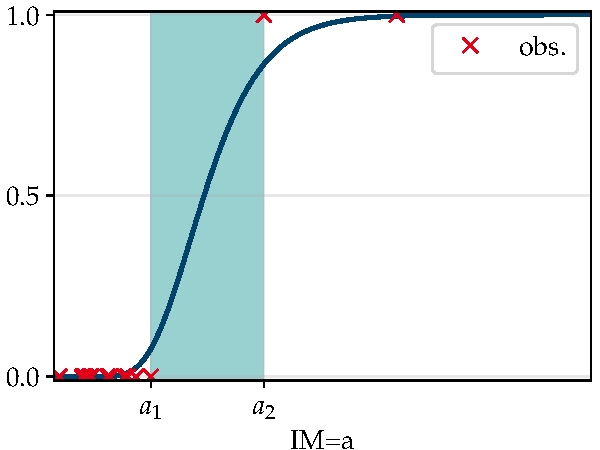
\includegraphics[width=4.44cm]{figures/PREM/degeneracy.pdf}
    \caption{{Example of a type 3 data sample $(\mbf z^k,\mbf a^k)$ which gives a degenerate likelihood. Graphs of (left) the likelihood given the degenerate data sample as a function of the tuple $(\alpha,\beta)$ and (right) the fragility curve (blue curve) according to which the points (red crosses) are sampled : each red cross is a tuple $(z,a)$, where its X-axis equals $a$ and its Y-axis equals $z$.}
    In both figures, $a_1$ is the maximal observed IM value among ``non-failures'', and $a_2$ is minimal one among ``failures''.
    The interval $(a_1,a_2)$ (in cyan in the right figure) separates the failures and the non-failure observed.
    }
    \label{fig:constr-frags:degenerate-frag}
\end{figure}



When the likelihood is degenerate, the vector $\mbf N$ is null and the likelihood does not shrink at $\beta\to0$.
As a consequence, the posterior will be proper only if the prior is proper w.r.t. $\beta$.
Moreover, in case of degeneracy of type 1 or 2, the likelihood does not shrink at either $\alpha\to\infty$ or $\alpha\to0$. In such a scenario, it becomes also essential to consider a prior that is proper  w.r.t. $\alpha$.

%Type 3
In practice, cases of degeneracy of type 1 and type 2 capture little attention. 
Indeed, it makes sense that when we work with binary data, an observation set containing only failure outcomes, or containing only non-failure outcomes does not allow estimating appropriately a fragility curve.
However, cases of degeneracy of type 3 are critical since they are likely to appear, especially when (i) the data are scarce, and (ii) the IM is more correlated with the system's response (see   \cref{app:chap:uncecomp}).


\section{Constrained reference prior for probit-lognormal fragility curves}\label{sec:constr-frags:constrained}


\subsection{Constrained reference prior framework}\label{sec:constr-frags:subsec-constr-frame}



To construct the prior, we take as a support the reference prior theory, whose principle is to maximize w.r.t. the prior the mutual information $\sI^k$. The mutual information is expected to measure the amount of information brought by the data over the \emph{a priori} information in the workflow. This methodology ensures the prior can be qualified as objective. We recall that this theory is completely reviewed in   \cref{chap:intro-ref}.
The mutual information can be written as a function of the prior $\varPi$:
\begin{equation}\label{eq:constr-frag:MI}
    \sI^k(\varPi) = \int_{\Theta}\int_{\cA^k}\sum_{\mbf z^k\in\{0,1\}^k}f\left(\frac{\int_\Theta\ell_k(\mbf z^k|\mbf a^k,\theta')d\varPi(\theta')  }{\ell_k(\mbf z^k|\mbf a^k,\theta)}\right)\ell_k(\mbf z^k|\mbf a^k,\theta)dH^{\otimes k}(\mbf a^k)d\varPi(\theta)  ,    
\end{equation}
where $f=-\log$ in the original theory, yet in this study we consider the mutual information written with $f=f_\delta:x\mapsto\frac{x^\delta-1}{\delta(\delta-1)}$, $\delta\in(0,1)$.
This corresponds to the generalized mutual information 
based on $\delta$-divergence, introduced in   \cref{chap:ref-generalized}. 

To be precise, the mutual information expression written in \cref{eq:constr-frag:MI} is not directly maximized w.r.t. $\varPi$, it is maximized asymptotically as $k\rightarrow\infty$ w.r.t. $\varPi$. We refer to   \cref{chap:intro-ref} or   \cref{chap:ref-generalized} for a more detailed definition of the reference prior. This asymptotic maximization is noted in this chapter as follows:
\begin{equation}\label{eq:constr-frag:optimnoconstr}
    \varPi^\ast\in\argmax_{\pi\in\cP;\,k\rightarrow\infty}\sI^k(\varPi),
\end{equation}
where $\cP$ is the set of all possible priors, namely the set of continuous $\sigma$-finite measures on $\Theta$.

It has been proven (see \cref{chap:intro-ref,chap:ref-generalized}) that the optimization problem~\eqref{eq:constr-frag:optimnoconstr} admits the Jeffreys prior as a solution. That prior is defined from its density $J$, expressed up to a constant as:
    \begin{equation}
        J(\theta)\propto\sqrt{|\det\cI(\theta)|}\quad\text{with}\quad \cI(\theta) = -\sum_{z\in\{0,1\}}\int_{\cA}\nabla_\theta^2\log\ell(z|a,\theta) \ell(z|a,\theta)dH(a).
    \end{equation}

As expressed in the introduction, we aim at applying the work done in   \cref{chap:constrained-prior}, in which it is suggested to add a constraint in the optimization problem~\eqref{eq:constr-frag:optimnoconstr}:
\begin{equation}\label{eq:constr-frag:optimconstr}
    \varPi^\ast\in\argmax_{\varPi\in\cP;\,k\rightarrow\infty}\sI^k(\varPi),\quad\text{subject to\ }\cC(\varPi)<\infty,
\end{equation}
where $\cC(\varPi)= \int a(\theta)d\varPi(\theta)$ for some function $a(\cdot)$.
That function is sought to regularize the Jeffreys prior decay rates. If it verifies
    \begin{equation}\label{eq:constr-frag:inta}
        \int_\Theta J(\theta)a(\theta)^{1+1/\delta}d\theta <\infty, \quad\text{and} \quad \int_\Theta J(\theta)a(\theta)^{1/\delta}<\infty 
    \end{equation}
then the prior whose density is proportional to $\theta\mapsto J(\theta)\cdot a^{1/\delta}(\theta)$ is the solution of problem~\eqref{eq:constr-frag:optimconstr}, and is a proper prior.


\subsection{Application to the probit-lognormal reference prior}\label{sec:constr-frags:subsec-constr-in-probit}


In   \cref{chap:prem}, the Jeffreys prior decay rates have been comprehensively studied.
We recall that
% \begin{equation}
    \begin{align}\label{eq:constr-frag:decaysJbeta}
        &\forall\alpha>0,\, J(\theta) \aseq{\beta\rightarrow0}\frac{D'(\alpha)}{\beta}\quad\text{and}\quad J(\theta)\aseq{\beta\rightarrow\infty}\frac{E'}{\alpha\beta^3}, \\
        &\forall\beta>0,\,J(\theta) \aseq{\log\alpha\rightarrow\pm\infty}G''(\beta)\frac{|\log\alpha|}{\alpha}\exp\left(-\frac{(\log\alpha-\mu)^2}{2\beta^2+2\sigma^2}\right),\label{eq:constr-frag:decaysJalpha}
    \end{align}
% \end{equation}
where $D'(\alpha)>0$ depends only on $\alpha$, $E'>0$ is a constant, and $G''(\beta)>0$ depends only on $\beta$.

The Jeffreys prior has an improper tail at $\beta\to0$ which does not shrinks when it is multiplied by a degenerate likelihood.
% This asymptotic rate at $\beta\to0$ is actually 
While we do not exactly know the shape of the prior on the whole domain, we assume that we can associate it to (i) an improper marginal distribution w.r.t. $\beta$ whose density follows asymptotically the rates in \cref{eq:constr-frag:decaysJbeta}, and (ii) a proper distribution of $\alpha$ conditionally to $\beta$.



It is thus possible to construct a constraint that will adjust the decay rate at $\beta\to0$ of the Jeffreys prior in order to make it integrable.
We chose $a(\theta)=\theta^\kappa$, that satisfies \cref{eq:constr-frag:inta} for $\kappa\in(0,\frac{2\delta}{1+\delta})$. 
The solution of the optimization problem~\eqref{eq:constr-frag:optimconstr} is then the prior whose density $\pi^\ast$ verifies $\pi^\ast(\theta)\propto J(\theta)\beta^{\kappa/\delta}$. In this work, we denote by $\varPi^\ast_\gamma$ this prior and by $\pi^\ast_\gamma$ its density, where $\gamma:=\kappa/\delta\in(0,\frac{2}{1+\delta})\subset(0,2)$:
    \begin{equation}
        \pi^\ast_\gamma(\theta) \propto J(\theta)\beta^\gamma.
    \end{equation}


%A little regularization of that decay rates allows to make it integrable.







%In our problem 


% \subsection{Theoretical expression of the prior}


\subsection{Practical derivation with integral interpolations}\label{sec:constr-frags:subsec-practical-interpol}


%In this section, we briefly recall the derivation process of the Jeffreys prior and 
The prior $\varPi_\gamma^\ast$ can be implemented by approximating numerically its density $\pi^\ast_\gamma$, using the theoretical expression of the Jeffreys prior.
We recall that, in   \cref{chap:prem}, we proved that %Jeffreys' density can be expressed as 
the Fisher information matrix can be expressed as 
\begin{equation}
    %\label{eq:infmat}
        \cI(\theta)=\begin{pmatrix}
        \frac{1}{\alpha^2\beta^2}(A_{01} + A_{02}) & \frac{1}{\alpha\beta^3}(A_{11}+A_{12}) \\
        \frac{1}{\alpha\beta^3}(A_{11}+A_{12}) & \frac{1}{\beta^4}(A_{21}+A_{22})
    \end{pmatrix},
    \end{equation}
by defining 
$A_{01}$, $A_{02}$, $A_{11}$, $A_{12}$, $A_{21}$, $A_{22}$ as
    \begin{equation} %\label{eq:Aij}
    \begin{aligned}
        %A_{11} &= \int_\cA\Phi'(\gamma)d\PP_A(a) & A_{12} &= \int_\cA\log\frac{a}{\alpha}\Phi'(\gamma)d\PP_A(a) \\
        A_{0u} &= \int_\cA\frac{\Phi'(\beta^{-1}\log\frac{a}{\alpha})^2}{\Phi((-1)^{u+1}\beta^{-1}\log\frac{a}{\alpha})}h(a)da,\\
        %& A_{02} &= \int_{\cA}\frac{\Phi'(\beta^{-1}\log\frac{a}{\alpha})^2}{\Phi(-\beta^{-1}\log\frac{a}{\alpha})}p(a)da,\\
        A_{1u} &= \int_\cA\log\frac{a}{\alpha}\frac{\Phi'(\beta^{-1}\log\frac{a}{\alpha})^2}{\Phi((-1)^{u+1}\beta^{-1}\log\frac{a}{\alpha})}h(a)da,\\
        %& A_{12} &= \int_{\cA}\log\frac{a}{\alpha}\frac{\Phi'(\beta^{-1}\log\frac{a}{\alpha})^2}{\Phi(-\beta^{-1}\log\frac{a}{\alpha})}p(a)da,\\
        A_{2u} &= \int_\cA\log^2\frac{a}{\alpha}\frac{\Phi'(\beta^{-1}\log\frac{a}{\alpha})^2}{\Phi((-1)^{u+1}\beta^{-1}\log\frac{a}{\alpha})}h(a)da,
        %& A_{22} &= \int_{\cA}\log^2\frac{a}{\alpha}\frac{\Phi'(\beta^{-1}\log\frac{a}{\alpha})^2}{\Phi(-\beta^{-1}\log\frac{a}{\alpha})}p(a)da,\\
    \end{aligned}
    \end{equation}
%reminding $\gamma=\beta^{-1}\log\frac{a}{\alpha}$.
for $u\in\{1,2\}$, and where $h$ denotes the p.d.f. of the IM.
%It is then 

Using the above, it is possible to approximate $J(\theta)$ by conducting Simpson's interpolations of the involved integrals in the Fisher information matrix. The interpolations are performed from a large dataset of IM values. We refer to   \cref{chap:frags-intro} where the seismic signal generator used in this work to provide
a large dataset of seismic signals is presented. The empirical distribution of the PGA of the seismic signals in that dataset is recalled in \cref{fig:constr-frags:PGA}. %That generator has been used to construct a dataset of $10^5$ seismic signals for which different IMs have been derived.
The interpolations are done a regular grid of $\cA=[a_{\min},a_{\max}]$, where $a_{\min}$ (resp. $a_{\max}$) is the minimal (reps. the maximal) value of the IM in the dataset.
The density $h$ is approximated by Gaussian kernel density estimation. 

Due to the computational cost of the numerical interpolations involved when approximating the Jeffreys prior, we conducted the same methodology as in   \cref{chap:prem}. This methodology consists in evaluating it on an experimental design based on a fine-mesh grid $\Theta$. These evaluations allow building an interpolated approximation of the Jeffreys prior density matching the design.
The density $\pi^\ast_\gamma$ is then obtained by multiplying the interpolated approximated Jeffreys by $\beta^\gamma$.

\begin{figure}[h]
    \centering
    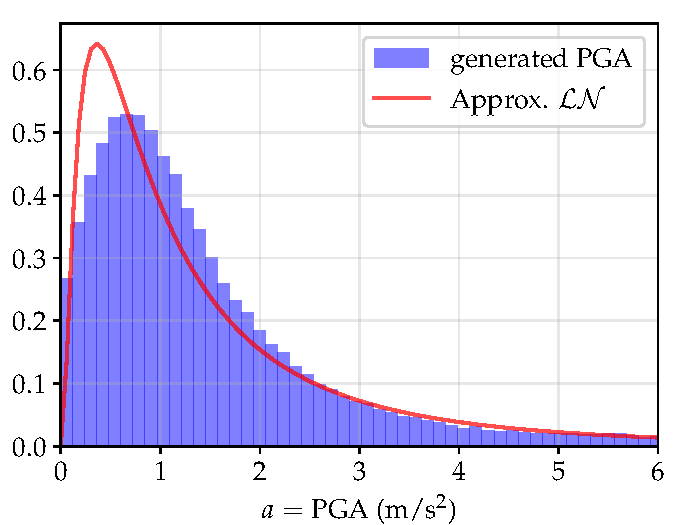
\includegraphics[width=5.2cm]{figures/constr-frags/pgadistrib.pdf}
    \label{fig:constr-frags:PGA}
    \caption{%
    Comparison of the histograms of the PGA values of generated signals (blue) with a lognormal
    density (red) that has same median (i.e. $0$) and same log deviation (i.e. $1$).}
    %approximations (red) for both IMs (PSA in the left figure, PGA in the right figure).}
\end{figure}





\section{Variational approximation of the constrained reference prior}\label{sec:constr-frags:varp}


\subsection{Definition of the VA-RP}\label{sec:constr-frags:subsec:varpdef}

The second approximation of the constrained reference prior that we conduct results form a variational inference methodology.
We recall that
variational inference encompasses a range of techniques designed to approximate probability distributions by solving an optimization problem (such as maximizing the evidence lower bound, as in \cite{kingma_auto-encoding_2014}). 
%For more information about variational inference, we refer to   \cref{chap:varp}.
Since our goal is to find
%Given that our objective involves finding 
the prior that maximizes the mutual information defined in \cref{eq:constr-frag:MI}, variational inference naturally lends itself to the approximation of reference priors.  

The approach that we conduct is based on the variational approximation of the reference prior (VA-RP) proposed in   \cref{chap:varp}.
It consists in limiting the family of priors to a parametric class $\{\varPi_\lambda,\,\lambda\in\Lambda\}$, with $\Lambda\subset\mathbb{R}^L$, thereby reducing the problem to a finite-dimensional setting. Consequently, the optimization tasks in equations \cref{eq:constr-frag:optimnoconstr,eq:constr-frag:optimconstr} %(  {eq:RPdef}) and (  {eq:def_const_RP}) 
translate into maximizing $\sI^k(\varPi_\lambda)$ over $\lambda\in\Lambda$. We define the priors $\varPi_\lambda$ implicitly through the transformation:
\begin{equation}
    \theta \sim \varPi_{\lambda} \iff \theta = g(\lambda,\varepsilon), \quad \text{where} \quad \varepsilon \sim \PP_{\varepsilon}.
\end{equation}
Here, $g$ is a parameterized measurable function ---typically a neural network--- where $\lambda$ represents its weights and biases, it has to be differentiable with respect to $\lambda$. The variable $\varepsilon$ serves as a latent variable, drawn from a simple, easy-to-sample distribution $\PP_\eps$. In practice, we choose a centered multivariate Gaussian $\mathcal{N}(0,I_{p\times p})$.  














\subsection{Optimization under constraints}\label{sec:constr-frags:subsec:optim}


The VA-RP is sought to approximate the solution of the optimization problems~\eqref{eq:constr-frag:optimnoconstr} or~\eqref{eq:constr-frag:optimconstr}.

To do so, the problem is considered for a fixed value of $k$. 
Also, instead of maximizing the mutual information, the method is maximizes the following objective function, which is a lower bound of the mutual information:
    \begin{equation}
        \lambda^\ast\in\argmax_{\lambda\in\Lambda} \cB^k(\varPi_\lambda),\quad \cB^k= \EE_{\theta\sim\varPi_\lambda}\sum_{\mbf z^k\in\{0,1\}^k}\int_{\cA^k}f_\delta\left(\frac{\ell_k(\mbf z^k|\mbf a^k,\hat\theta^{\text{MLE}})}{\ell_k(\mbf z^k|\mbf a^k,\theta)}\right) \ell_k(\mbf z^k|\mbf a^k,\theta)h(a)da,
    \end{equation}
where $\hat\theta^{\text{MLE}}$ refers to the maximum likelihood estimator: $\ell_k(\mbf z^k|\mbf a^k,\hat\theta^{\text{MLE}}) = \max_{\theta\in\Theta}\ell_k(\mbf z^k|\mbf a^k,\theta) $.


The optimization is conducted by stochastic gradient ascent, provided that the gradient of the objective function $\cB^k$ w.r.t. $\lambda$ is given by
    \begin{equation}
        \EE_{\eps\sim\PP_\eps}\left[\sum_{j=1}^{2}\partial_{\theta_j}\tilde\cB^k(g(\lambda,\eps))\nabla_\lambda g_j(\lambda,\eps)
        \right],
    \end{equation}
where the gradients of the neural network $\nabla_\lambda g(\lambda,\eps)$ are computed in the algorithm via automatic differentiation, and the terms $\partial_{\theta_j}\tilde\cB^k(g(\lambda,\eps))$  depend on the likelihood of % explicitly derived for 
the probit-lognormal model:
    \begin{equation}
        \partial_{\theta_j}\tilde\cB^k(\theta) = \sum_{\mbf z^k\in\{0,1\}^k}\int_{\cA^k} \partial_{\theta_j}\log\ell_k(\mbf z^k|\mbf a^k,\theta) F_\delta\left(\frac{\ell_k(\mbf z^k|\mbf a^k,\hat\theta^{\text{MLE}})}{\ell_k(\mbf z^k|\mbf a^k,\theta)}\right)\ell_k(\mbf z^k|\mbf a^k,\theta)h(a)da,
    \end{equation}
where $F_\delta(x) = f_\delta(x)-xf_\delta'(x)$.
The derivatives of the log-likelihood here equal the following:
    \begin{equation}
        \begin{aligned}
            &\partial_\alpha\log\ell_k(\mbf z^k|\mbf a^k,\theta) =  -\frac{1}{\alpha\beta}z\frac{\Phi'(\beta^{-1}\log\frac{a}{\alpha})}{\Phi(\beta^{-1}\log\frac{a}{\alpha})} + \frac{1}{\alpha\beta}(1-z)\frac{\Phi'(\beta^{-1}\log\frac{a}{\alpha})}{1-\Phi(\beta^{-1}\log\frac{a}{\alpha})} , \\
            &\partial_\beta\log\ell_k(\mbf z^k|\mbf a^k,\theta) = -\frac{\log\frac{a}{\alpha}}{\beta^2}z\frac{\Phi'(\beta^{-1}\log\frac{a}{\alpha})}{\Phi(\beta^{-1}\log\frac{a}{\alpha})}+ \frac{\log\frac{a}{\alpha}}{\beta^2}(1-z)\frac{\Phi'(\beta^{-1}\log\frac{a}{\alpha})}{1-\Phi(\beta^{-1}\log\frac{a}{\alpha})} .
        \end{aligned}
    \end{equation}



%The gradient ascent algorithm can be ad

Still following the method of   \cref{chap:varp},
the gradient ascent algorithm is adapted to approximate explicitly the solution of the optimization problem~\eqref{eq:constr-frag:optimconstr}.
This adaptation consists in actually solving
    \begin{equation}
        \lambda^\ast\in\argmax_{\lambda\in\Lambda}\cB^k(\varPi_\lambda)\quad\text{subject to\ } \cC(\varPi_\lambda)=0,
    \end{equation}
where $\cC(\varPi_\lambda)=\int_\Theta a(\theta)d\varPi_\lambda(\theta) - c/\cK$, with
    \begin{equation}
        \cK=\int_\Theta J(\theta)a(\theta)^{1/\delta}d\theta \quad\text{and}\quad
        c = \int_\Theta J(\theta)a(\theta)^{1+1/\delta}d\theta.
    \end{equation}
The above constants are derived using the numerical approximation of the Jeffreys prior density proposed in \cref{sec:constr-frags:subsec-practical-interpol}.
For more details on the conduction of the optimization process, we refer to   \cref{chap:varp}.



\subsection{Neural network architecture}\label{sec:constr-frags:architecture}


A single layer neural network is implemented for this problem. It takes the following form
\begin{equation}\label{eq:neuralnet-architecture}
    \eps \mapsto \begin{pmatrix}
        \mbf t_1(\eps)\\ \mbf t_2(\eps) 
    \end{pmatrix} \mapsto
          %
    \begin{pmatrix}
        \tilde\eps_1 = \mbf w_1^\top\mbf t_1(\eps) + b_1 \\
        \tilde\eps_2 = \mbf w_2^\top\mbf t_2(\eps)+b_2 
    \end{pmatrix} \mapsto
    \begin{pmatrix}
        \alpha = u_1(\tilde\eps_1)\\
        \beta = u_2(\tilde\eps_2)
    \end{pmatrix}.
\end{equation}
The coordinates of the vectors $\mbf w_1,\mbf w_2\in\RR^p$ and $\mbf b=(b_1,b_2)\in\RR^2$ constitute the weights of the neural network, they are initialized independently and randomly w.r.t. a Gaussian distribution. $\mbf t_1$, $\mbf t_2$, $u_1$, $u_2$ are activation functions.
They are specifically chosen in order to ensure the VA-RP's decay rates match with the ones of the target prior: $u_1=u_2=\exp$ and for $\mbf x\in\RR^p$, $\mbf t_1(\mbf x)=(t_1(x_i))_i$ and $\mbf t_2(\mbf x)=(t_2(x_i))_i$ with
\begin{equation}
    t_1(x) = x;\quad t_2(x) = \log(1-\Phi(x)),
\end{equation}
%where $\Phi$ designates the c.d.f. of a standard Gaussian.
In appendix~\ref{sec:constr-frags:app}, we prove that under those settings the VA-RP yields marginal distributions $ p_\alpha$, $p_\beta$ w.r.t. $\alpha$, $\beta$, that take the following form:
    \begin{equation}
        \begin{aligned}
        p_\alpha(\alpha) &= \frac{1}{\alpha\sqrt{2\pi}\|\mbf w_1 \|_2}\exp\left(-\frac{(\log\alpha - b_1)^2}{2\|\mbf w_1\|^2_2}\right) \\
        p_\beta(\beta) &= \sum_{i,\, w_{2i}>0}{K_i}\beta^{-\frac{1}{w_{2i}}-1}\indic_{\beta>e^{b_2}} + \sum_{i,\, w_{2i}<0}K_i\beta^{-\frac{1}{w_{2i}}-1}\indic_{\beta<e^{b_2}},
    \end{aligned}
    \label{eq:marginaldist}
    \end{equation}
where $(w_{2i})_{i=1}^p$ denote the coordinates of $\mbf w_2$, and the $K_i$ are constants that depend on $\mbf w_2$ and $b_2$. 
The marginal distribution $p_\alpha$ is a log-normal distribution, which is similar, up to the $\log \alpha$ term, to the Jeffreys prior decay rates w.r.t. $\alpha$ (\cref{eq:constr-frag:decaysJalpha}).  Concerning $p_\beta$, calling $w_{2j}^{-1}=\min\{w_{2i}^{-1},\,w_{2i}>0\}$ and $w_{2l}^{-1}=\max\{w_{2i}^{-1},\,w_{2i}<0\}$, 
it admits the following decay rates:
\begin{equation}
    p_\beta(\beta)\equi{\beta\rightarrow0} K_j\beta^{-\frac{1}{w_{2l}}-1};\quad p_\beta(\beta)\equi{\beta\rightarrow\infty} K_l\beta^{-\frac{1}{w_{2j}}-1}.
    \label{eq:palphabeta}
\end{equation}
They are consistent with the ones of the Jeffreys prior. % (resp. the $\gamma$-constrained Jeffreys prior), if $\frac{1}{w_{2j}}$









%we approximate the solution of the constrained optimization problem (\cref{eq:constr-frag:optimconstr}) by solving the optimization problem





% \subsection{Posterior sampling}

%This implicit construction provides considerable flexibility in defining prior distributions. However, except in simpler cases, the density function of $\pi_\lambda$ remains unknown and cannot be evaluated directly. Instead, we obtain samples $\theta\sim\pi_\lambda$.  








\section{Comparison between the VA-RP and the interpolated reference prior}\label{sec:constr-frags:coparisonpriors}


% \subsection{}

In this section, we compare the approximation of the target prior using the VA-RP approach with the approximation by numerical interpolation of the theoretical expression of the Jeffreys prior density (denoted AJ).
We consider that the AJ is a more accurate approximation of the target than the VA-RP. For this reason, this section mostly serves the assessment of the VA-RP methodology in the context of the probit-lognormal model.

We implemented the probit-lognormal modeling assuming that the p.d.f. h of the IM is defined by
%We have implemented the probit-lognormal modeling by setting the p.d.f. $h$ of the IM as
    \begin{equation}\label{eq:constr-frags:ha}
        h(a) = \frac{1}{\sqrt{2\pi}\sigma_a^2 a}\exp\left(-\frac{(\log a-\mu_a)^2}{2\sigma_a^2}\right)
    \end{equation}
with
$\mu_a=0$ and $\sigma_a=1$. These parameters, which define the distribution of $a$, are the only elements that have a theoretical impact on the reference prior.
Their value are derived to fit the empirical distribution of the PGA values of the seismic signals that we consider. That empirical distribution is compared with the p.d.f. of \cref{eq:constr-frags:ha} in \cref{fig:constr-frags:PGA}.
%Their values are derived from the case study which is considered in \cref{sec:constr-frags:appasg}.
%  Section~{sec:case-study}.





\paragraph{Training of the unconstrained VA-RP}
First, we present the training process of the unconstrained VA-RP. It is expected to approach the unconstrained reference prior, i.e. the Jeffreys prior. 
%The latter being improper, we expect the training to 
% irregularities 
% The 
As for the different parameters 
for the training, we take $k=50$ and $p=50$. The training consists in the maximization of $\cB^k$ with $\delta=0.5$. 
The optimization has been done through a number of $9000$ epochs, with a learning rate of $0.005$.


\Cref{fig:unconstr_weights} shows the evolutions of the weights of the neural network that define the marginal distributions of $p_\alpha$ and $p_\beta$ (see \cref{eq:marginaldist}), as a function of the number of epochs. Thus, the bias $b_1$ is constant and equal to $0$, which is consistent with the asymptotic distribution of $\alpha$. $1/w_{2l}$ and $1/w_{2j}$ both tend to $0$. As a result, the marginal distribution of $\beta$ tends to $1/\beta$. This is an improper distribution which does not exactly match the expected improper Jeffreys prior (see \cref{eq:constr-frag:decaysJbeta}): it has a heavier tail as $\beta\to\infty$ than the original Jeffreys. 
However, we will see at the end of this section that the information contained in the distribution is not concentrated in its tails. In reality, low values of $\beta$ have huge weights
%However, we will see in the end of this section that the distribution is not limited to its tails, and that this prior actually ascribes huge weights to small values of $\beta$ 
(see the paragraph ``Posterior evaluation''). Finally, $\|\mbf w_1\|_2$ tends to $+\infty$. This means that the variance of  $\log\alpha$ tends to $+\infty$ as it is expected (see appendix~\ref{sec:constr-frags:app}), even though this does not lead to the target distribution. This last result is nevertheless not surprising. It is the consequence of the chosen architecture of the VA-RP: $p_\alpha$ is a lognormal distribution (\cref{eq:palphabeta}), which is not exactly the case for the Jeffreys prior (\cref{eq:constr-frag:decaysJalpha}). What fundamentally distinguishes these two distributions is that (i) in the first case, that of Jeffreys, the variance of $\log\alpha$ is finite conditionally to $\beta$, and is infinite otherwise because of the heavy tail of the distribution w.r.t. $\beta$ %is infinite because of the heavy tail of the distribution
while (ii) in the second case, the variance becomes infinite to correspond, via the training process, to the target variance of the Jeffreys prior. In doing so, the marginal distribution of $\alpha$ tends towards the improper distribution $1/\alpha$. Although this result is open to criticism, it appears to be an ``acceptable'' compromise insofar as the model's likelihood tends to substantially attenuate the prior's tails with respect to $\alpha$, thereby limiting the influence of the prior's decay rates on the posterior. An alternative approach could involve modifying the neural network architecture to better capture the correlation between $\alpha$ and $\beta$. However, such adjustments would inevitably increase the computational complexity of the training process.


\begin{figure}[h]
    \centering
    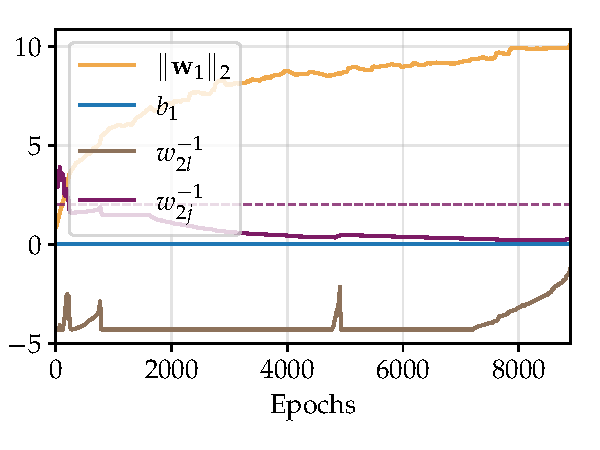
\includegraphics[width=5.2cm]{figures/constr-frags/weights_unconstr.pdf}
    \caption{
        Weights of interest of the neural network during the unconstrained optimization. %The yellow and blue curves represent respectively $\|\mbf w_1 \|_2$ and $|b_1|$, where $\|\mbf w_1 \|_2^2$ is the variance of the log of the first component, and $b_1$ its mean. 
    The brown and violet curves represent respectively $1/w_{2l}$ and $1/w_{2j}$ that are defined in \cref{sec:constr-frags:architecture}. In violet dashed line is plotted the target value of $1/w_{2j}$. % plotted their target value.
    %Parameters of interest of the neural network during the unconstrained optimization. The yellow and blue curves represent respectively $\|\mbf w_1 \|_2$ and $|b_1|$, where $\|\mbf w_1 \|_2^2$ is the variance of the log of the first component, and $b_1$ its mean. The brown and violet curves represent respectively $1/w_{2l}$ and $1/w_{2j}$ which appear in the decay rates of the second component.
    }
    \label{fig:unconstr_weights}
\end{figure}



\paragraph{Training of the constrained VA-RP}
As for the constrained case, we remind that we introduce a constraint of the form $\cC(\varPi_\lambda)=0$ with  $\cC(\varPi_\lambda) = \int_\Theta \beta^\kappa d\varPi_\lambda - \cK/c$.
We fix $\kappa=0.15$, so that $\gamma=\kappa/\delta=0.3$.
In this case the VA-RP is expected to approximate the constrained reference prior, i.e. the prior whose density  $\pi^\ast$ is proportional to $\theta\mapsto J(\theta)\beta^\gamma$.
Its asymptotic rates are identical to those of the Jeffreys prior for $\alpha$. If we fix $\alpha$, we have then:
\begin{equation} 
\begin{cases} \displaystyle
\pi^\ast(\theta) \propto \beta^{\gamma -1} \quad \text{as} \quad  \beta \longrightarrow 0 \\
\pi^\ast(\theta) \propto \beta^{\gamma - 3} \quad \text{as} \quad  \beta \longrightarrow +\infty.
\end{cases} 
\end{equation} 
In this case, the development done in the appendix~\ref{sec:constr-frags:app} suggests that this prior verifies $\EE_{\theta\sim\pi^\ast}|\log\alpha|^2=\infty$.
The training process of the constrained VA-RP is done during $12000$ epochs with a learning rate of $0.001$. %We take $N=50$, $T=50$ and $p=50$. the parameter $\eta$ in the augmented Lagrangian is updated every $10$ epochs.



\Cref{fig:constr-frags:training-constr}.(a) suggests that the constraint seems reasonably verified during the whole optimization as the constraint gap is close to zero and appears to be decreasing. \Cref{fig:constr-frags:training-constr}(b) shows that the inverse weights $1/w_{2l}$ and $1/w_{2j}$ appear to steadily approach their theoretical values, respectively $-\gamma=-0.3$ and $2-\gamma = 1.7$. As in the unconstrained case, we observe that $\|\mbf w_1\|_2$ tends to $+\infty$. This is consistent with the theoretical results of \cref{sec:var_prior_alpha} which suggest, recall, that for all $\gamma\geq0$, $\EE[|\log\alpha|^2]=\infty$. So, we verify that adding constraints therefore allows, as expected, to ``control'' the distribution of $\beta$. Concerning $\alpha$, we find the same trend as in the unconstrained case, which is theoretically expected from the point of view of the variance of the marginal distribution.


\begin{figure}[h]
    \centering
    %\begin{tabular}{@{}c@{}}		
	%\subfloat[Constraint value gap. \label{fig:constr_gap}]
    {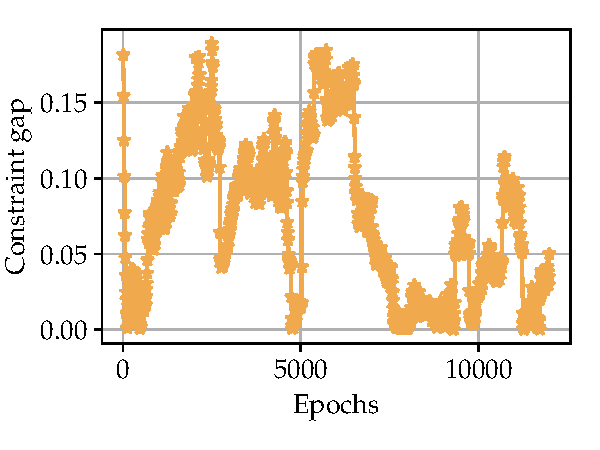
\includegraphics[width=5.2cm]{figures/constr-frags/constraint gap.pdf}}
    %\end{tabular}
    %\hspace{-0.2cm}    
    %\begin{tabular}{@{}c@{}}		
	%\subfloat[Weights of interest of the neural network. \label{fig:constr_weights} ]
    {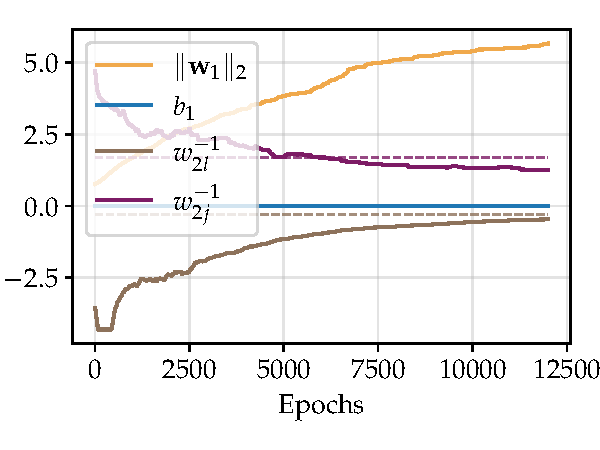
\includegraphics[width=5.2cm]{figures/constr-frags/weights_constr.pdf}}
    \makebox[5.2cm]{(a)}\makebox[5.2cm]{(b)}
    %\end{tabular}
  \caption{(a) Evolution of the constraint value gap during training. It corresponds to the difference between the target and current values for the constraint (in absolute value). (b) Weights of interest of the neural network during the constrained optimization. The yellow and blue curves represent respectively $\|\mbf w_1 \|_2$ and $b_1$, where $\|\mbf w_1 \|_2^2$ is the variance of the log of the first component, and $b_1$ its mean. The brown and violet curves represent respectively $1/w_{2l}$ and $1/w_{2j}$ that are defined in \cref{sec:constr-frags:architecture}. In same color dashed line are plotted their target value.\label{fig:constr-frags:training-constr}}
% \label{fig:constr_gap_weights}    
\end{figure}

%str_weights}
%\end{figure}

\paragraph{Posterior evaluation}
We evaluate the posterior that the VA-RPs derived in this section yield.
For this purpose, we take as dataset $k=50$ samples $(\mbf z^k,\mbf a^k)$, $\mbf z^k=(z_i)_{i=1}^k$, $\mbf a^k=(a_i)_{i=1}^k$, that are generated given a probit-lognormal model with $\theta_{\text{true}}$ close to $(3.37, 0.43)$. %The distribution of. % considered is still a log-normal with $\mu_a=0$ and $\sigma_a=1$.

\emph{A posteriori} samples are generated for both approaches by using an adaptive Metropolis-Hasting (M-H).
In the case of the AJ approach, the M-H is implemented to generate samples using the approximated posterior density.
In the case of the VA-RP, the M-H is implemented to generate samples using the posterior density $q(\cdot|\mbf z^k,\mbf a^k)$ density of $\eps$:
    \begin{equation}
        q(\eps|\mbf z^k,\mbf a^k) \propto q(\eps)\ell_k(\mbf z^k|\mbf a^k,g(\lambda,\eps)),
    \end{equation}
where $q(\cdot)$ denotes the p.d.f. of $\eps$.
\emph{A posteriori} samples of $\theta$ are obtained by applying the neural network $g(\lambda,\cdot)$ to the \emph{a posteriori} samples of $\eps$.
For both methods, a number of $5000$ samples of $\theta$ are generated this way.
In this example, 
we precise that the likelihood is not degenerate.
% For the sake of completeness, they are compared with samples generated considering an other prior: the actual reference prior derived by approximating numerically its theoretical expression, as depicted in \cite{van2024reference}. 
% The samples are generated by an other adaptive Metropolis-Hastings algorithm, which iteratively evaluates the prior. In the following, we refer to the latter as AJ.

%For the posterior, we take as dataset $50$ samples from the probit model with $\theta_{true}$ close to $(3.37, 0.43)$. The adaptive Metropolis-Hastings algorithm on $\varepsilon$ is applied for $10^5$ iterations, the last $5000$ a posteriori samples are kept. 


%We would like to avoid the situation where the data points are partitioned into two disjoint subsets when classified according to $a$ values. In that case, the posterior becomes improper because the likelihood is constant (\cite{van2024reference}), we say that the dataset is degenerate.


%we have not retained the samples for which the data are dissociated into two disjoint subsets when they are classified according to the values of $a$. In this case, indeed, the posterior distribution is improper because the likelihood is constant when $\beta$ tends to 0 \cite{van2024reference}. We then say that the dataset is degenerate \cite{AVB2025}. The probability of occurrence of such datasets is not negligible if the dataset has a small size. The following plots are obtained with non-degenerate datasets. 


\begin{figure}[h]
    \centering
    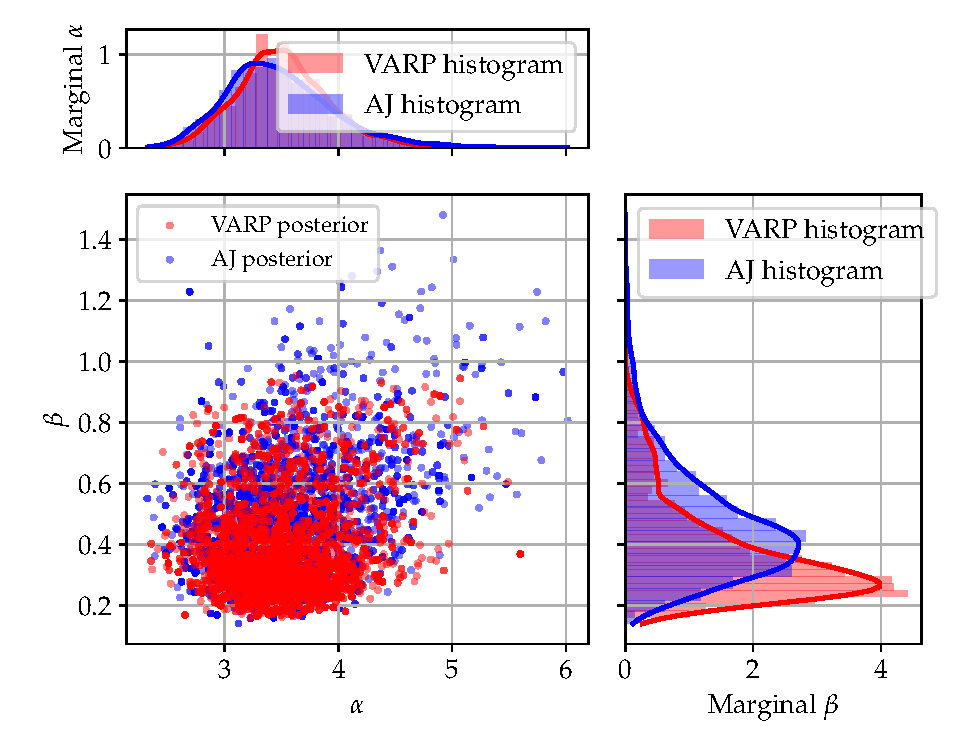
\includegraphics[height=7cm]{figures/constr-frags/hist_post_marg_unconstrained_new.pdf}%
    \caption{Scatter histogram of the unconstrained VA-RP posterior and the approximated Jeffreys (AJ)  posterior distributions obtained from $5000$ samples. Kernel density estimation is used on the marginal distributions in order to approximate their density functions with Gaussian kernels.}
    \label{fig:scatterhist_unconstr}
\end{figure}

\begin{figure}[h!]
    \centering
    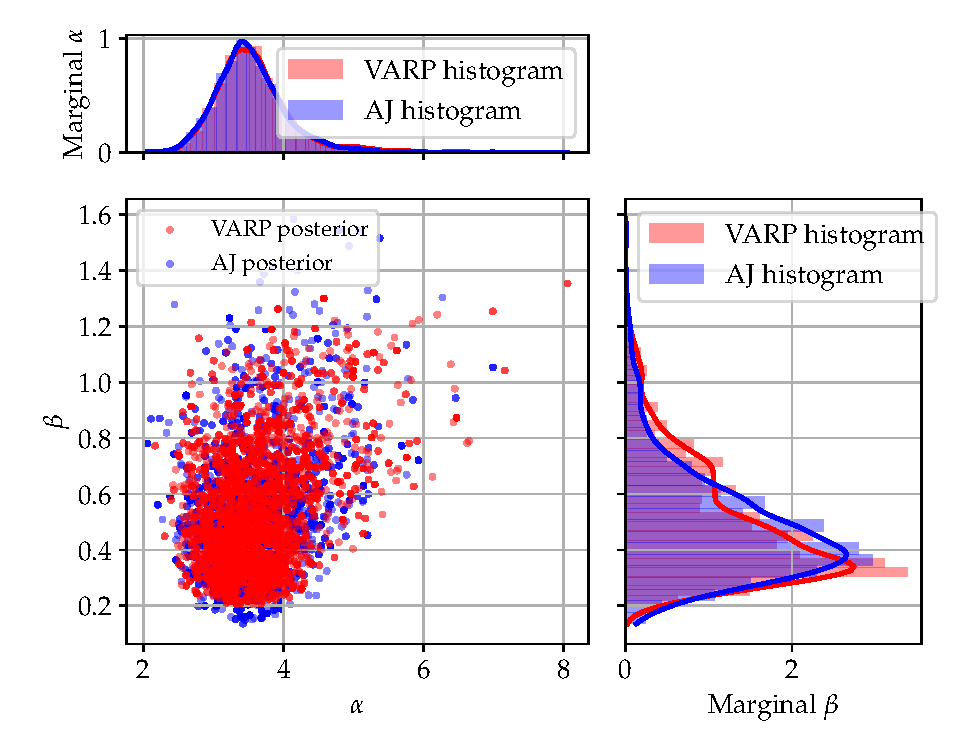
\includegraphics[height=7cm]{figures/constr-frags/hist_post_marg_constrained_new.pdf}
    \caption{Scatter histogram of the constrained VA-RP posterior and the approximated Jeffreys (AJ)  posterior distributions obtained from $5000$ samples. Kernel density estimation is used on the marginal distributions in order to approximate their density functions with Gaussian kernels.}
    \label{fig:scatterhist_constr}
\end{figure}



\Cref{fig:scatterhist_unconstr,fig:scatterhist_constr} show that the posterior distribution obtained from the VA-RP looks more like Jeffreys prior %more closely resembles to the Jeffreys prior 
in the constrained case than in the unconstrained one. 
More specifically, w.r.t. $\alpha$, the VA-RP is similar to the Jeffreys prior in both cases. That suggests that the limitation of our neural network architecture discussed earlier has little impact on the posterior distribution.
Regarding $\beta$,
in the unconstrained case, the VA-RP ascribes predominant weight to smaller values of $\beta$ compared to the Jeffreys prior, with a mode that is closer to $0$. In terms of fragility curve estimation that could represent an issue, as it may lead to estimates with thinner credibility intervals around a fragility curve. %that approximates an ---irrealistic--- unit-step function.









\section{Application of the method on a case study}\label{sec:constr-frags:appasg}


In this section, we propose to apply the VA-RP that we have constructed and optimized above
% in what precedes 
to an industrial problem.
The industrial problem, described in the following subsection, consists in a piping system that was introduced in   \cref{chap:frags-intro} (\cref{sec:intro-frags:casstudies}). 
This application serves as a proof of concept, we intend to show that the constrained VA-RP allows estimating efficiently and accurately seismic fragility curves in practice.








\subsection{Case study description as a reminder}\label{sec:constr-frags:subsec:asgdesc}


The studied mechanical system consists in a piping system that comes from the secondary cooling circuit of a French pressurized water reactor.
The piping was presented in details in   \cref{chap:frags-intro} (\cref{sec:intro-frags:piping}) and is illustrated in \cref{fig:constr-frag:asg}.
The mock-up has submitted to artificial seismic signals on a shaking table that permits to validate a finite element model, which simulates the structure's response under seismic excitations.
A total of $8\cdot 10^4$ nonlinear dynamical simulations have been carried out given seismic signals that were taken from the dataset of $10^5$ signals that we dispose. These results serve as a validation dataset. 
The engineering demand parameter (EDP) for this structure corresponds to the out-of-plane rotation of its first elbow (see the details in   \cref{chap:frags-intro}), the results of the simulations are plotted in the plan (PGA,EDP) in \cref{fig:constr-frag:asg}-middle.
In \cref{fig:constr-frag:asg}-right, reference fragility curves given different rotation threshold are derived for this structure. They are computed using the non-paramteric method proposed by \citet{trevlopoulos_parametric_2019} and detailed in   \cref{chap:frags-intro} (\cref{sec:intro-frags:subsec-nonparametric}).






\begin{figure}[h]
    \centering
    \parbox[b][3.8cm][c]{4.5cm}{%
    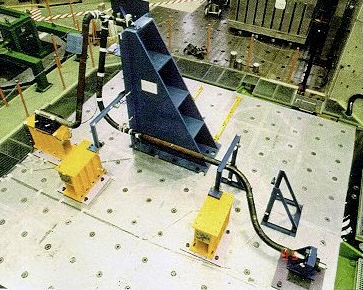
\includegraphics[height=3.2cm]{figures/intro-frags/ASG.jpg}\vspace*{1em}%
    }
    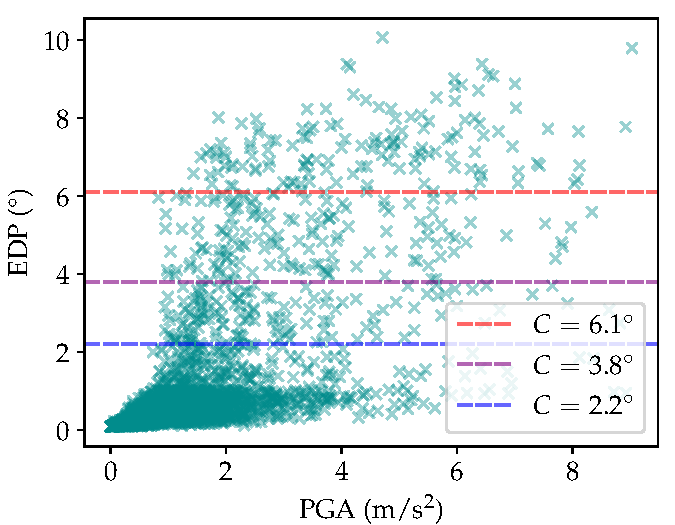
\includegraphics[height=3.8cm]{figures/intro-frags/asg/cloud_PGA_light.pdf}\ \ 
    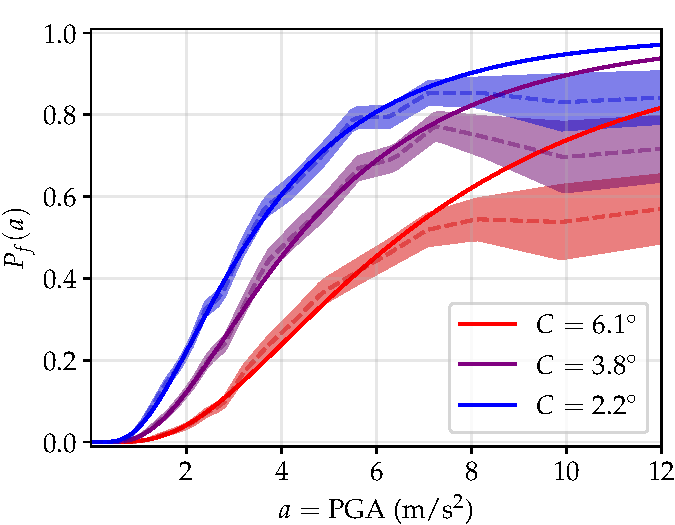
\includegraphics[height=3.8cm]{figures/intro-frags/asg/refs_PGA.pdf}
    \caption{Illustration of the case study. Left: picture of the mock-up on the Azalee shaking table of CEA. Middle: results of $8\cdot10^4$ non-linear dynamical simulations. Right: reference non-parametric fragility curves (dashed lines) surrounded by their $95\%$-confidence intervals, compared with the probit-lognormal fragility curves derived by MLE from the validation dataset of size $10^5$. Different threshold $C$ are considered, each yields different proportions of failures in the validation dataset: resp. $95\%$ (red), $90\%$ (purple) and $85\%$ (blue).}
    \label{fig:constr-frag:asg}
\end{figure}



\subsection{Benchmarking metrics}\label{sec:constr-frags:subsec:benchmarking}


In this chapter, we evaluate our estimates by comparing them to a reference fragility curve $P^{\text{ref}}_f$. As explained in the previous subsection, the reference is computed using a non-paramteric method implemented from the available validation dataset of $8\cdot 10^4$ samples.

In \cref{fig:constr-frag:asg},
different fragility curves, derived considering different excessive rotation threshold for defining the equipment's failure are elucidated. 
In this study, the failure of the system was defined when the EDP exceeded $C=3.8^\circ$.
%in Figure~  {fig:refs}.
The reference $P^{\text{ref}}_f$ is compared to a probit-lognormal curve $P^{\text{MLE}}_f$ whose parameters are estimated by maximum likelihood estimation using the same validation dataset.
%Each are compared with a probit-lognormal curve $P^{\text{MLE}}_f$, derived implementing a maximum likelihood estimate of the probit-lognormal fragility curve using the full batch of the $8\cdot 10^4$ results depicted in Figure~  {fig:cloud_data}. 
That comparison demonstrates the adequacy of such modeling of the fragility curve. However, it also emphasizes an existing bias that the model has compared with the non-parametric estimate. In the following, we refer to this difference between $P_f^{\text{MLE}}$ and $P_f^{\text{ref}}$ as the square model bias, denoted by $\cM\cB$:
\begin{equation}
    \cM\cB = \|P^{\text{ref}}_f - P^{\text{MLE}}_f  \|_{L^2}^2;
\end{equation}
where the norm $\|\cdot \|_{L^2}$ is defined by $\|P\|_{L^2}^2=\int_{a_{\min}}^{a_{\max}} P(a)^2da$ where the domain $[a_{\min},a_{\max}]
$ covers the available seismic signals. The norm is derived numerically from Simpson's interpolation. % on a regular sub-division of $(0,\infty)$.




Given an observed sample of size $k$: $(\mbf z^k,\mbf a^k)$, $\mbf z^k=(z_i)_{i=1}^k$, $\mbf a^k=(a_i)_{i=1}^k$, we denote by $P_f^{|\mbf z^k,\mbf a^k}:a\mapsto \Phi(\beta^{-1}\log (a/\alpha))$ the process whose distribution inherits from the posterior distribution  of $\theta$ conditionally to $(\mbf z^k,\mbf a^k)$. For any value of $a$, we note $q_{r}^{|\mbf z^k,\mbf a^k}(a)$ the $r$-quantile of $P^{|\mbf z^k,\mbf a^k}_f(a)$, and $m^{|\mbf z^k,\mbf a^k}(a)$ its median.
We propose to evaluate our estimates using the following metrics:
\begin{itemize}
    \item The square bias to the median $\cB^{|\mbf z^k,\mbf a^k}=\|m^{|\mbf z^k,\mbf a^k}-P^{\text{ref}}_f\|^2_{L^2}$.
    \item The square credibility width $\cW^{|\mbf z^k,\mbf a^k}=\|q_{1-r/2}^{|\mbf z^k,\mbf a^k} - q_{r/2}^{|\mbf z^k,\mbf a^k}\|^2_{L^2}$, with $r=0.05$.
    \item The upper quantile error $\cQ^{|\mbf z^k,\mbf a^k}=\|q_{1-r/2}^{\mbf z^k,\mbf a^k}-P_f^{\text{ref}} \|^2_{L^2}$.
\end{itemize}
%
% For comparison purpose, we suggest to derive the above metrics 
The quantiles and the medians are approximated using generated samples.









\subsection{Results}\label{sec:constr-frags:subsec:results}




%In this section, we compare the evaluation of our estimates that results from using the VA-RP with the evaluation of the ones that result from using an approximation via numerical derivation of the Jeffreys prior. In the following, we refer to the latter as AJ.
%Both are implemented with and without the incorporation of a constraint that is tailored to ensure they are proper. The considered constraint is detailed in Section~  {sec:varp-implementation}.


In \cref{fig:frag-ex-asg} we provide examples of \emph{a posteriori} fragility curves credibility intervals yielded by the two priors, with and without incorporating a constraint on the decay rates.
These examples arise from given samples of $k=80$ observations. They illustrate that the VA-RP is capable of providing fragility curve estimates that are equivalent of the ones provided by the AJ, which is an approximation of the exact expression of the reference prior.


\begin{figure}[h]
    \centering
    % \begin{tabular}{@{}c@{}}		
	% \subfloat[\label{fig:ex_ASG_unconstr50}]{
    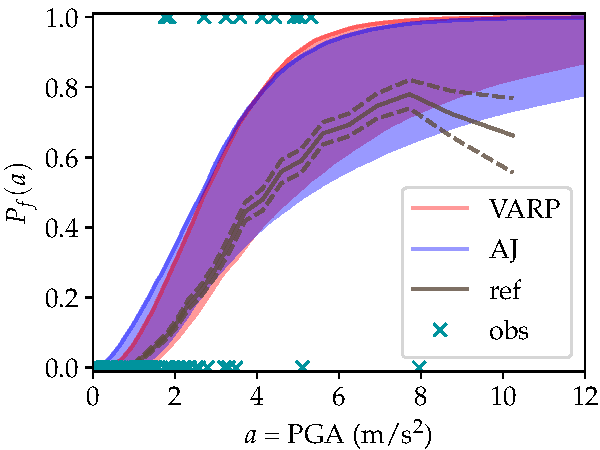
\includegraphics[width=5cm]{figures/constr-frags/ex_ASG_unconstr80.pdf}\ %}
    % \end{tabular}
    % \hspace{0.1cm}
    % \begin{tabular}{@{}c@{}}		
	%\subfloat[\label{fig:ex_ASG_constr50}]{
    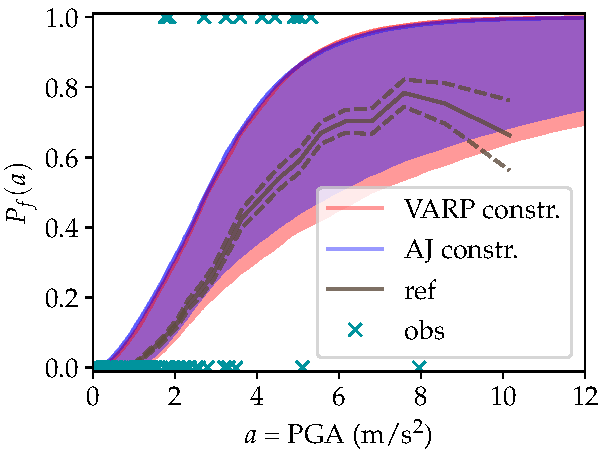
\includegraphics[width=5cm]{figures/constr-frags/ex_ASG_constr80.pdf}\\%
    \makebox[5cm]{(a)}\ \makebox[5cm]{(b)}
    % \end{tabular}
    \caption{Example of \emph{a posteriori} $95\%$ credibility intervals yielded by the posterior distribution resulting from a sample of $k=80$ data and from the VA-RP (in red) or the AJ (in blue)~: (a) unconstrained priors and (b) constrained priors.
    The reference curve $P^{\text{ref}}_f$ (solid line) is surrounded by its $95\%$ confidence interval (dashed line) in each figure. The cyan crosses represent the observed sample.}
    \label{fig:frag-ex-asg}   
\end{figure}



To deepen the comparison, 
we implemented the methods multiple times for values of $k$ varying in $[10,250]$. More precisely, for each $k\in\{10,20,\dots,250\}$, $10$ random data samples of size $k$ have been drawn. Each of these samples were then used to compute the metrics $\cB^{|\mbf z^k,\mbf a^k}$, $\cW^{|\mbf z^k,\mbf a^k}$ and $\cQ^{|\mbf z^k,\mbf a^k}$.

The average values of these metrics along with their $95\%$ confidence intervals are presented in \cref{fig:errors-unconstrained} (for the unconstrained case) and \cref{fig:errors-constrained} (for the constrained case) as functions of $k$.






\Cref{fig:errors-unconstrained,fig:errors-constrained} confirm previous results on a larger scale, namely that, with the current architecture, the constrained VA-RP outperforms the unconstrained VA-RP. Regarding bias, for example, it produces less erratic results. Compared to the AJ approximation, the VA-RP approximations exhibit slightly larger biases. The gap decreases as the number of data increases as expected, but only in the constrained case. Regarding the sizes of the credibility intervals (the values of $\cW^{|\mbf z^k,\mbf a^k}$), they are generally smaller in the unconstrained case. This result is consistent with the observation made in \cref{fig:scatterhist_unconstr} concerning the marginal distribution of $\beta$. This shows smaller values than with the AJ approximation of the Jeffreys prior.
It is important to emphasize that it is primarily the lower bounds of the credibility intervals that are ``penalized'' with the constrained VA-RP approximation. The upper bound remains consistent with that of the AJ, as reflected in the values of $\cQ^{|\mbf z^k,\mbf a^k}$. This result illustrates the relevance of using the constrained VA-RP approach for safety study. Indeed, in such a context, focusing on the upper quantile is consistent with a conservative approach.







\begin{figure}[h]
    \centering
    \makebox[0pt]{%
    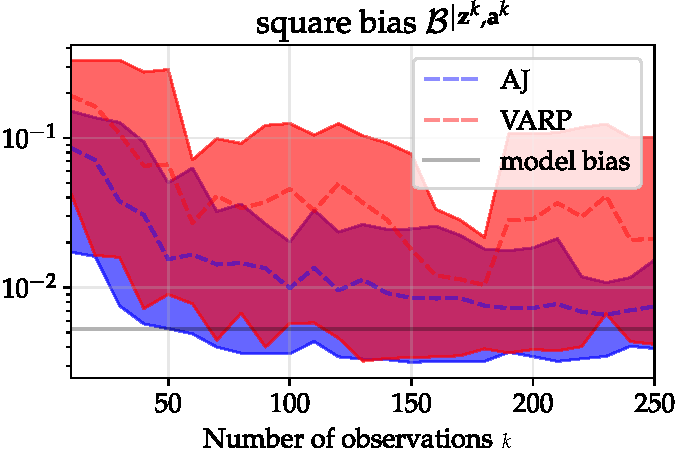
\includegraphics[width=5cm]{figures/constr-frags/errB_n.pdf}%
    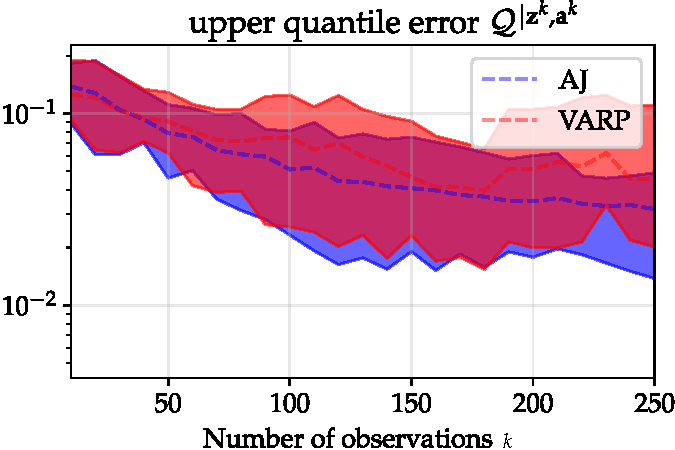
\includegraphics[width=5cm]{figures/constr-frags/errQ_n.pdf}%
    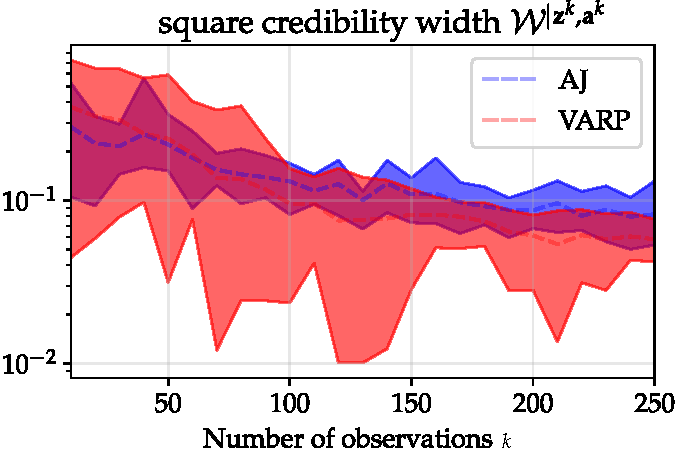
\includegraphics[width=5cm]{figures/constr-frags/errW_n.pdf}%
    }
    \caption{Average errors (dashed line) $\cB^{|\mbf z^k,\mbf a^k}$, $\cQ^{|\mbf z^k,\mbf a^k}$, $\cW^{|\mbf z^k,\mbf a^k}$ and their $95\%$ confidence intervals, derived from numerical replications of the unconstrained methods for each value of $k$ in $\{10,20,\cdots,250\}$. The values derived 
    using the VA-RP (red) are compared with the ones 
    using a numerical derivation to approximate the Jeffreys prior (blue). In the left figure, the square model bias $\cM\cB$ is plotted (solid line).}
    \label{fig:errors-unconstrained}
\end{figure}




\begin{figure}[h]
    \centering
    \makebox[0pt]{%
    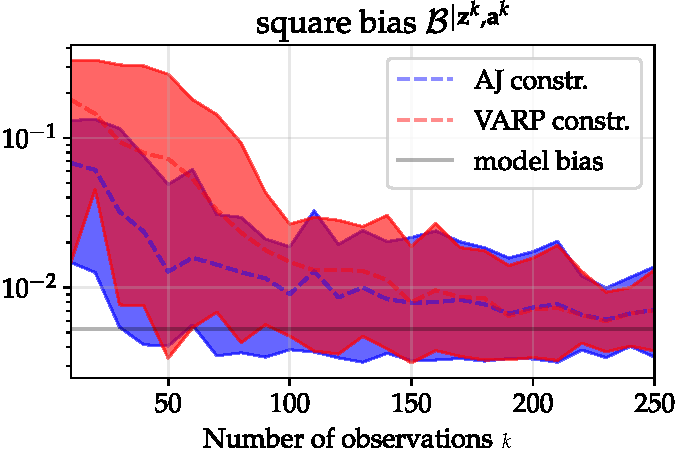
\includegraphics[width=5cm]{figures/constr-frags/errB_c.pdf}%
    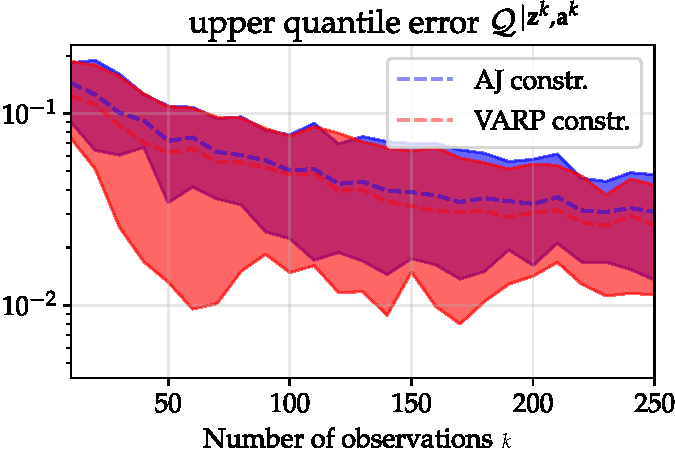
\includegraphics[width=5cm]{figures/constr-frags/errQ_c.pdf}%
    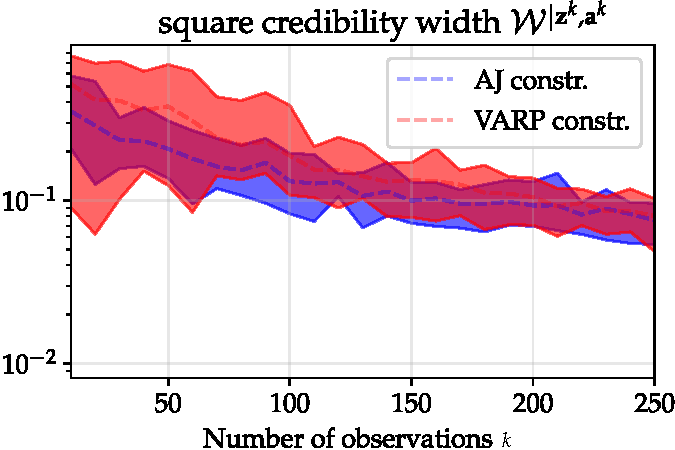
\includegraphics[width=5cm]{figures/constr-frags/errW_c.pdf}%
    }
    \caption{Same as \cref{fig:errors-unconstrained}, but when a constraint is incorporated in the priors.}
    \label{fig:errors-constrained}
\end{figure}









\section{Appendix: impacts of the neural network's architecture on the VA-RP}\label{sec:constr-frags:app}




\subsection{Decay rates of the VA-RP density}\label{app:decay-rates}

In this appendix we elucidate the form taken by the marginal distribution of the VA-RP w.r.t. $\beta$.
The VA-RP is assumed to be expressed as presented in \cref{sec:constr-frags:architecture} (\cref{eq:neuralnet-architecture}): the random variable $\beta$ is defined as
    \begin{equation}\label{eq:app-expr-beta}
        \beta = \exp\left[\sum_{i,\,w_{2i}\ne0}w_{2i}\log(1-\Phi(\eps_i)) + b_i\right],
    \end{equation}
where the $(\eps_i)_i$ are independent standard Gaussian variables.
%As the weights $(w_{2i})_i$ are initialized 
We recall that the weights $(w_{2i})_{i}$ are initialized randomly w.r.t. a Gaussian distribution. Therefore, they have almost surely 
% we reasonably suppose that they have 
distinct absolute values.
We rely on the two following lemmas.
\begin{lem}\label{lemma:expon-distrib}
    Let $X$ be a random variable following a standard Gaussian distribution, and $\mu>0$. Then
    \begin{itemize}
        \item the r.v. $Z=-\mu^{-1}\log(1-\Phi(X))$ admits the density $f_Z$ defined by $f_Z(z)=\mu e^{-\mu z}\indic_{z>0}$, it is an exponential distribution with parameter $\mu$;
        \item the r.v $\tilde Z=\mu^{-1}\log(1-\Phi(X))$ admits the density $f_{\tilde Z}$ defined by $f_{\tilde Z}(z)= \mu e^{\mu z}\indic_{z<0}$, we call it an opposite exponential distribution with parameter $-\mu$.
    \end{itemize}
\end{lem}
\begin{lem}\label{lemma:sum-of-expon}
    Let $Z_1,\dots,Z_n$ be independent exponential or opposite exponential distribution with parameters $(\mu_{i})_{i=1}^n$, distinct in absolute value. Their sum $\overline{Z}$ admits a density $f_{\overline{Z}}$ that takes the form
        \begin{equation}\label{eq:lem-pdf-Z}
            f_{\overline{Z}}(z) = \sum_{i,\,\mu_i>0}K_ie^{-\mu_i z}\indic_{z>0} + \sum_{i,\,\mu_i<0}K_ie^{-\mu_iz}\indic_{z<0},
        \end{equation}
    for some constants $K_1,\dots,K_n$.
\end{lem}


The expression of $\beta$ as written in \cref{eq:app-expr-beta} expresses $\log(\beta-b_2)$ as a sum of independent exponential or opposite exponential distributions with parameters $(|w_{2i}|^{-1})_{i}$, which are distinct.
Thus, the r.v. $\log(\beta-b_2)$ admits a density $\tilde p$ that is defined as in \cref{eq:lem-pdf-Z}:
\begin{equation}
    \tilde p(z) = \sum_{i,\,w_{2i}>0}K_ie^{-\frac{z}{w_{2i}}}\indic_{z>0} + \sum_{i,\,w_{2i}<0}K_ie^{-\frac{z}{w_{2i}}}\indic_{z<0}.
\end{equation}
Given that $p_\beta(\beta e^{b_2})e^{b_2}\propto\tilde p(\log\beta) / \beta$ there exists some constants $(\tilde K_i)_{i=1}^n$ such that
\begin{equation}
    p_\beta(\beta) = \sum_{i,\,w_{2i}>0}\tilde K_i\beta^{-\frac{1}{w_{2i}}-1}\indic_{\beta>e^{b_2}} + \sum_{i,\,w_{2i}<0}\tilde K_i\beta^{-\frac{1}{w_{2i}}-1}\indic_{\beta<e^{b_2}}.
\end{equation}


\begin{proof}[{Proof of \cref{lemma:expon-distrib}}]
First, $\Phi$ being the c.d.f. of a standard Gaussian distribution, $\Phi(X)$ follows an uniform distribution in $(0,1)$.
The density $f_Z(z)=\frac{e^{-\frac{z}{\mu}}}{\mu}$ involved in the first statement of the lemma is the p.d.f. of an exponential distribution with parameter $\mu^{-1}$. The c.d.f. of that distribution is defined by $F_Z(z) = -\mu\log(1-z)$.
Thus, $-\mu\log(1-\Phi(X))$ is an exponential distribution with parameter $\mu^{-1}$.\\
To conclude, notice that the second statement of the lemma simply results by elucidating the p.d.f. of $\tilde Z$ from the one of $Z$ given that $\tilde Z=-Z$.
\end{proof}



\begin{proof}[{Proof of \cref{lemma:sum-of-expon}}]
We prove this result by induction over $n$. When $n=1$, the form in \cref{eq:lem-pdf-Z} is consistent with the p.d.f. of an exponential or opposite exponential distribution.

We suppose this statement true for $n-1$ such r.v., we denote by $\tilde f$ the p.d.f. of $\sum_{i=1}^{n-1}Z_i$, and by $f_{Z_n}$ the one of $Z_n$. As $\sum_{i=1}^{n-1}Z_i$ and $Z_n$ are independent, $f_{\overline{Z}}$ equals the convolution between $\tilde f$ and $f_{Z_n}$: $f_{\overline{Z}}=\tilde f\ast f_{Z_n}$.

Before going further, let us derive the following integrals, for any $0<\nu_1<\nu_2$:
\begin{align}
        \nonumber&\int_\RR e^{-\nu_1(y-x)}e^{-\nu_2 x}\indic_{y-x>0}\indic_{x>0}dx = \frac{e^{-\nu_2 y}-e^{-\nu_1 y}}{\nu_2-\nu_1}\indic_{y>0},\\
        %
        &\int_\RR e^{-\nu_1(y-x)}e^{\nu_2 x}\indic_{y-x>0}\indic_{x<0} dx = \frac{e^{\nu_2y}}{\nu_1+\nu_2}\indic_{y<0} + \frac{e^{-\nu_1y}}{\nu_1+\nu_2}\indic_{y>0},\\
        %
        %& \int_\RR e^{-\nu_1(y-x)}e^{-\nu_1 x} \indic_{y-x>0}\indic_{x>0}dx = ye^{-\nu_1 y} \indic_{y>0} \\
        %
        %& \int_\RR e^{\nu_1(y-x)}e^{\nu_1 x}\indic_{y-x<0}\indic_{x<0}dx = 
        %
        &\int_\RR e^{\nu_1(y-x)}e^{\nu_2 x}\indic_{y-x<0}\indic_{x<0}dx = \frac{e^{\nu_1y} - e^{\nu_2y}}{\nu_2-\nu_1}\indic_{y<0}.\nonumber
    \end{align}
Thus, if $f_{Z_n}(x) = \mu_n e^{-\mu_n x}\indic_{x>0}$ for  $\mu_n>0$ we get
    \begin{align}
        f_{\overline{Z}}(z) =&  \sum_{i<n,\,\mu_i>0} \frac{K_i\mu_n}{\mu_i-\mu_n}e^{-\mu_i z}\indic_{z>0}  + \sum_{i<n,\,\mu_i<0}\frac{K_i\mu_n}{\mu_i+\mu_n}e^{-\mu_i z}\indic_{z<0}
        \\
        &- e^{-\mu_n z}\left[\sum_{i,\,\mu_i>0}\frac{K_i\mu_n}{\mu_i-\mu_n} + \sum_{i,\,\mu_i<0}\frac{K_i\mu_n}{\mu_i+\mu_n} \right]\indic_{z>0};\nonumber
    \end{align}
and if $f_{Z_n}(x) = \mu_n e^{\mu_n x}\indic_{x<0}$ for  $\mu_n>0$ then 
    \begin{align}
        f_{\overline{Z}}(z) =&  \sum_{i,\,\mu_i>0} \frac{K_i\mu_n}{\mu_i+\mu_n}e^{-\mu_i z}\indic_{z>0}  + \sum_{i,\,\mu_i<0}\frac{K_i\mu_n}{\rho-\mu_n}e^{-\mu_i z}\indic_{z<0}\\
        &+ e^{\mu_n z}\left[\sum_{i,\,\mu_i>0}\frac{K_i\mu_n}{\mu_i+\mu_n} + \sum_{i,\,\mu_i<0}\frac{K_i\mu_n}{\mu_i-\mu_n} \right]\indic_{z<0}.\nonumber
    \end{align}
In any case, it fits the expected form.
\end{proof}

\subsection{Variance of $\log\alpha$ a priori}
    \label{sec:var_prior_alpha}



In this section, we assume that the constrained reference prior has a density that takes the following form:
\begin{equation}
    \pi^\gamma(\theta) = p(\alpha|\beta)p^\gamma(\beta),\quad p(\alpha|\beta)\propto \frac{|\log\alpha|}{\alpha}\exp\left(-\frac{(\log\alpha-\mu)^2}{2\beta^2+2\sigma^2}\right),\quad p^\gamma(\beta) \propto\frac{1}{\beta^{1-\gamma}+\beta^{3-\gamma}},
\end{equation}
where $\mu\in\RR$, $\sigma>0$, and $\gamma\in(0,2)$ that is null if the reference prior is not constrained.
The prior corresponds to (i) a marginal distribution w.r.t. $\beta$ that has the same decay rates as the theoretical target, and (ii) a distribution of $\alpha$ conditionally to $\beta$ whose decay rates corresponds to the ones in \cref{eq:constr-frag:decaysJalpha}.
We recall that $\gamma\in(0,2)$.



% In this section we consider the asymptotic version of the reference prior, that we denote by $\pi^{\gamma}_a$:
%     \begin{equation}
%         \pi^\gamma_a(\theta) = \frac{K}{\beta^{1-\gamma}+\beta^{3-\gamma}}\frac{|\log\alpha|}{\alpha}\exp\left(-\frac{(\log\alpha-\mu)^2}{2\beta^2+2\sigma^2}  \right), 
%     \end{equation}
% where $\mu\in\RR$, $\sigma>0$. The parameter $\gamma$ is non-null if the reference prior is not constrained, it lives  in $(0,2)$ if a constraint is incorporated as elucidated in \cref{sec:constr-frags:constrained}. $K$ represents a normalization constant that depends only on $\gamma$.

We fix $\beta>0$, let us consider a random variable $X\sim\cN(\mu,\Sigma^2)$, where $\Sigma=\Sigma(\beta) = \sqrt{\sigma^2+\beta^2}$. We can write
    \begin{align}
       &\EE|X| = \int_{-\infty}^\infty  \frac{|x|}{\sqrt{2\pi\Sigma^2}}e^{-\frac{(x-\mu)^2}{2\Sigma^2}}dx = \frac{1}{\sqrt{2\pi\Sigma^2}} \int_0^\infty \frac{|\log y|}{y}e^{-\frac{(\log y-\mu)^2}{2\Sigma^2}}dy\label{eq:app2-|x|}\\
       \text{and}\quad &
            \EE|X|^3 = \int_{-\infty}^\infty  \frac{|x|^3}{\sqrt{2\pi\Sigma^2}}e^{-\frac{(x-\mu)^2}{2\Sigma^2}}dx = \frac{1}{\sqrt{2\pi\Sigma^2}} \int_0^\infty \frac{|\log y|^3}{y}e^{-\frac{(\log y-\mu)^2}{2\Sigma^2}}dy.
    \end{align}
\Cref{eq:app2-|x|} elucidates the conditional distribution of $\alpha|\beta$ as the one whose density is
    \begin{equation}
        p^\gamma_a(\alpha|\beta) = (\EE|X|\sqrt{2\pi\Sigma^2})^{-1}\frac{|\log\alpha|}{\alpha} \exp\left(-\frac{(\log\alpha-\mu)^2}{2\beta^2+2\sigma^2}  \right).
    \end{equation}
% and the marginal distribution of $\beta$ as the one whose density is
    % \begin{equation}
    %     p_a^\gamma(\beta) = \frac{K(\EE|X|\sqrt{2\pi\Sigma^2})}{\beta^{1-\gamma}+\beta^{3-\gamma}} .
    % \end{equation}
This way,
    \begin{equation}\label{eq:app-Elog2|beta}
        \EE[|\log\alpha|^2\,|\,\beta] = \frac{\EE|X|^3}{\EE|X|}.
    \end{equation}
To derive the right-hand term of the above equation, we use the following (see \cite{winkelbauer_moments_2014}):
    \begin{equation}
        \begin{aligned}
        &\EE|X|^3 =  2^{3/2}\Sigma^3 \frac{\Gamma(2)}{\Gamma(-\frac{3}{2})} \sum_{k=0}^\infty \frac{\Gamma(-\frac{3}{2}+k)}{\Gamma(\frac{1}{2}+k)}\frac{\left(-\frac{\mu}{2\Sigma^2}\right)^k}{k!}, \\
        \text{and}\quad& 
            \EE|X| =  2^{1/2}\Sigma \frac{\Gamma(1)}{\Gamma(-\frac{1}{2})} \sum_{k=0}^\infty \frac{\Gamma(-\frac{1}{2}+k)}{\Gamma(\frac{1}{2}+k)}\frac{\left(-\frac{\mu}{2\Sigma^2}\right)^k}{k!}.
        \end{aligned}
    \end{equation}
Using the identity $z\Gamma(z)=\Gamma(z+1)$, we derive 
    \begin{equation}
        \frac{\Gamma(-\frac{3}{2}+k)}{\Gamma(\frac{1}{2}+k)} = \frac{\Gamma(-\frac{1}{2}+k)}{(-\frac{3}{2}+k)\Gamma(\frac{1}{2}+k)}= \frac{1}{(-\frac{3}{2}+k)(-\frac{1}{2}+k)}.
    \end{equation}
Going back to \cref{eq:app-Elog2|beta}, we deduce:
    \begin{equation}\label{eq:app-Elogalpha2-int}
        \EE|\log\alpha|^2 = \EE\left[\EE[|\log\alpha|^2\,|\,\beta]\right] = K'\int_0^\infty \frac{\beta^2+\sigma^2}{\beta^{1-\gamma}+\beta^{3-\gamma}}
        %\sum_{k=0}^\infty \frac{(-\mu(2\sigma^2+2\beta^2)^{-1})^k}{(2k-3)(2k-1)k!} 
        %d\beta,
        \frac{\sum_{k=0}^\infty \frac{(-\mu(2\sigma^2+\beta^2)^{-1})^k}{(2k-3)(2k-1)k!} }{\sum_{k=0}^\infty \frac{(-\mu(2\sigma^2+\beta^2)^{-1})^k}{-(2k-1)k!}}d\beta,
    \end{equation}
with $K'>0$ being a normalization constant.
To conclude, we perform an asymptotic analysis of the integrated function in the above equation as $\beta\to\infty$.
The power series 
    \begin{equation}
        \sum_{k=0}^\infty \frac{z^k}{(2k-3)(2k-1)k!} \quad\text{and}\quad 
        \sum_{k=0}^\infty \frac{z^k}{-(2k-1)k!}
    \end{equation}
have infinite radius of convergence, so that when $z\to0$, they converge respectively towards $\frac{1}{3}$ and $1$.
Also, while $z$ is a negative real number, the power series are positive.

Therefore, the term in the integral of \cref{eq:app-Elogalpha2-int} is positive and asymptotically equivalent to $\beta^{-1+\gamma}$ as $\beta\to\infty$. We deduce that for any $\gamma\geq0$,
    \begin{equation}
        \EE[|\log\alpha|^2]=\infty.
    \end{equation}
    





\section{Conclusion}\label{sec:constr-frags:conclusion}




In this work, we introduced a novel prior for conducting a Bayesian estimation of seismic fragility curves.
This prior results from the application of the development of the reference prior theory that we conducted in   \cref{part:ref-theory} of this manuscript.

First, we defined an appropriate constraint that regularizes the Jeffreys prior decay rates, in order to make it proper. In this way, the prior is ensured to yield proper posteriors, even in cases where the likelihood is degenerate.
Second, the prior was implemented using two approaches: one that is close to its theoretical expression, but that is computationally expensive to sample from; one that result from a variational approximation, which leads to a parameterized form of the prior that is more computationally efficient.
Third, the two approaches were compared and applied on a real case study. 
We believe that our results demonstrate that (i) the incorporated constraint provides an accurate and non-altered estimation of the fragility curves, and (ii) the VA-RP has been capable of accurately capturing the asymptotic behavior of the target prior, so that it provides competing estimates to the latter.

% and efficient me

Looking forward, %the VA-RP
% the architecture 
the impact that the chosen constraint has on the estimates requires further investigation. 
Such an investigation will be conducted in the following chapter, where the constrained reference prior that is suggested in this chapter will be implemented. %i%n 
















